\section{Experimental Plan}
\label{sec:experimentalPlan}
In the experiments, we want to study how batch incremental method of active learning works on the cifar-10 data-set and the data-set. For the classification model, we choose to use the VGG-net because it simplicity, short training time and powerful performance. The experiment will by conducts using Pytorch which is one of the most popular deep learning platform. 
The plan is first to compare the performance of different uncertainty base method. Then try the same thing with distance base method and BALD.



\section{Experimental Setup}

\label{sec:experimentalSetup}
For the first experiment, the active learner will query 100 instances for every 10 epoch of training. The training process will happens incrementally, where the size of the training set will gradually increase. Nearly all of the weight in the VGG-net will be initialized by using pre-trained weight, expect for the last three forward fully connected layer. The pre-trained weight is loaded from a pre-trained VGG model of ImageNet data-set which consist of 150,000 photographs and  1000 classes.




Optimizer Adam:
learning rate 0.0001, 
betas=(0.9, 0.999),
eps=1e-08, 

Graph1
Graph2
Graph3 making
\section{Experimental Results}

\label{sec:experimentalResults}
\subsection{Uncertainty base active learning}
\begin{figure}[!htb]%
    \centering
    \subfloat[]{{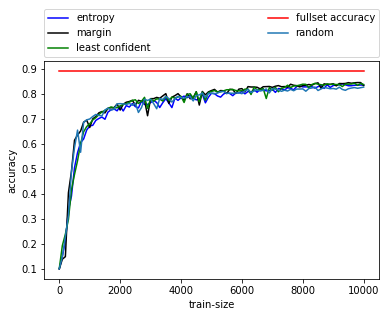
\includegraphics[width=5cm]{Contens/results/confident.png} }}%
    \qquad
    \subfloat[]{{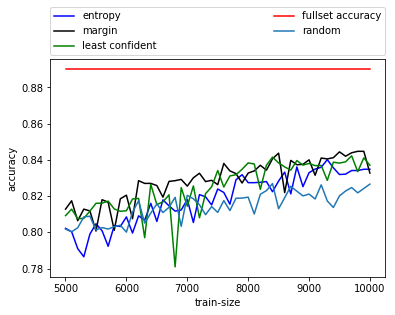
\includegraphics[width=5cm]{Contens/results/confident2.png} }}%
    \caption{Uncertainty base}%
    \label{fig:uncertainty1}%
\end{figure}
\subsection{BALD}

\begin{figure}[!htb]%
    \centering
    \subfloat[]{{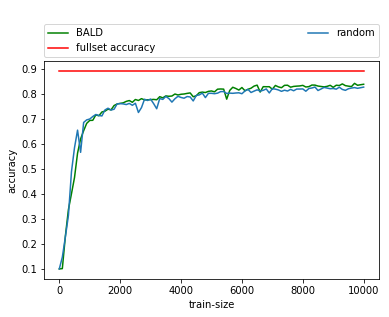
\includegraphics[width=5cm]{Contens/results/Bald1.png} }}%
    \qquad
    \subfloat[]{{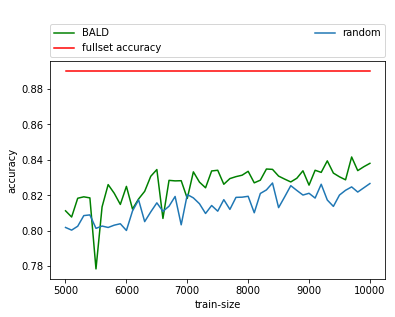
\includegraphics[width=5cm]{Contens/results/Bald2.png}.png} }%
    \caption{BALD}%
    \label{fig:BALD}%
\end{figure}
\subsection{Uncertainty base active learning}

Results should be clearly displayed and should provide a suitable representation of your results for the points you wish to make. Graphs should be labeled in a legible font and if more than one result is displayed on the same graph then these should be clearly marked.   Please choose carefully rather than presenting every results. Too much information is hard to read and often hides the key information you wish to present. Make use of statistical methods when presenting results, where possible to strengthen the results.  Further, the format of the presentation of results should be chosen based on what issues in the results you wish to highlight. You may wish to present a subset in the experimental section and provide additional results in the appendix.
\subsection{Least Confidence }
\subsection{Entropy Sampling}